% v2-acmsmall-sample.tex, dated March 6 2012
% This is a sample file for ACM small trim journals
%
% Compilation using 'acmsmall.cls' - version 1.3 (March 2012), Aptara Inc.
% (c) 2010 Association for Computing Machinery (ACM)
%
% Questions/Suggestions/Feedback should be addressed to => "acmtexsupport@aptaracorp.com".
% Users can also go through the FAQs available on the journal's submission webpage.
%
% Steps to compile: latex, bibtex, latex latex
%
% For tracking purposes => this is v1.3 - March 2012

\documentclass[prodmode,acmtecs]{acmsmall} % Aptara syntax

\usepackage{arydshln}
\usepackage{epsfig}
\usepackage{amsmath,amsfonts,amssymb,amstext}
\usepackage{natbib,multirow}
\usepackage{verbatimbox}
\usepackage{subfig}
\usepackage{epsfig}
% Package to generate and customize Algorithm as per ACM style
\usepackage[ruled]{algorithm2e}
\renewcommand{\algorithmcfname}{ALGORITHM}
\SetAlFnt{\small}
\SetAlCapFnt{\small}
\SetAlCapNameFnt{\small}
\SetAlCapHSkip{0pt}
\IncMargin{-\parindent}

% Metadata Information
\acmVolume{0}
\acmNumber{0}
\acmArticle{0}
\acmYear{0}
\acmMonth{0}

% Copyright
%\setcopyright{acmcopyright}
%\setcopyright{acmlicensed}
%\setcopyright{rightsretained}
%\setcopyright{usgov}
%\setcopyright{usgovmixed}
%\setcopyright{cagov}
%\setcopyright{cagovmixed}

% DOI
%\doi{0000001.0000001}

%ISSN
%\issn{1234-56789}

% Document starts
\begin{document}

% Page heads
\markboth{E. Irurozki et al.}{Algorithm xxx perm\_mateda: User's Manual}

% Title portion
\title{perm\_mateda: User's Manual}
\author{EKHINE IRUROZKI
\affil{Intelligent Systems Group, Basque Center for Applied Mathematics}
JOSU CEBERIO
\affil{Intelligent Systems Group, Faculty of Computer Science, University of the Basque Country UPV/EHU}
JOSEAN SANTAMARIA
\affil{Intelligent Systems Group, Faculty of Computer Science, University of the Basque Country UPV/EHU}
ROBERTO SANTANA
\affil{Intelligent Systems Group, Faculty of Computer Science, University of the Basque Country UPV/EHU}
ALEXANDER MENDIBURU
\affil{Intelligent Systems Group, Faculty of Computer Science, University of the Basque Country UPV/EHU}}




% NOTE! Affiliations placed here should be for the institution where the
%       BULK of the research was done. If the author has gone to a new
%       institution, before publication, the (above) affiliation should NOT be changed.
%       The authors 'current' address may be given in the "Author's addresses:" block (below).
%       So for example, Mr. Abdelzaher, the bulk of the research was done at UIUC, and he is
%       currently affiliated with NASA.

\begin{abstract}

This document describes how to install and use \texttt{perm\_mateda}, a Matlab package for the optimization of permutation problems. \texttt{perm\_mateda} is an extension of MATEDA-2.0, and it implements permutation-based probabilistic models (e.g. Mallows model) for different distances defined on permutations. The  package  is conceived for allowing the incorporation, by the user, of different combinations of selection, learning, sampling, and local search procedures. Similarly, additional permutation-based models can be added. Finally, the package includes the implementation of some of the most common permutation-based problems found in real-world applications. 
\end{abstract}

%
% The code below should be generated by the tool at
% http://dl.acm.org/ccs.cfm
% Please copy and paste the code instead of the example below. 
%

%\terms{Design, Algorithms, Performance}

\keywords{estimation of distribution algorithms, Mallows and Generalized Mallows models,  optimization, permutation-based problems, Matlab}

\acmformat{Ekhine Irurozki, Josu Ceberio, Josean Santamaria, Roberto Santana, Alexander Mendiburu, 2017. perm\_mateda: A matlab toolbox of estimation of distribution algorithms for permutation-based combinatorial optimization problems.}
% At a minimum you need to supply the author names, year and a title.
% IMPORTANT:
% Full first names whenever they are known, surname last, followed by a period.
% In the case of two authors, 'and' is placed between them.
% In the case of three or more authors, the serial comma is used, that is, all author names
% except the last one but including the penultimate author's name are followed by a comma,
% and then 'and' is placed before the final author's name.
% If only first and middle initials are known, then each initial
% is followed by a period and they are separated by a space.
% The remaining information (journal title, volume, article number, date, etc.) is 'auto-generated'.

\begin{bottomstuff}
This work has been partially supported by the Research Groups 2013-2018 (IT-609-13) and BERC 2014-2017 programs (Basque Government), and  TIN2016-78365-R and Severo Ochoa excellence accreditation SEV-2013-0323 programs (Spanish Ministry of Economy and Competitiveness).

Author's addresses: E. Irurozki, Basque Center for Applied Mathematics (BCAM), Alameda de Mazarredo 14, 48009 Bilbao, Bizkaia, Spain; J. Ceberio, J. Santamaria and R. Santana, Computer Science and Artificial Intelligence Department, Faculty of Computer Science, UPV/EHU, 20018 Paseo M. Lardizabal 1, Donostia - San Sebastian, Gipuzkoa, Spain; A. Mendiburu, Computer Architecture and Technology, Faculty of Computer Science, UPV/EHU, 20018 Paseo M. Lardizabal 1, Donostia - San Sebastian, Gipuzkoa, Spain.
\end{bottomstuff}

\maketitle

\section{Introduction}

Permutation problems are ubiquitous in the industry, society, and research. In transportation problems, sequence alignment, scheduling, or ranking determination, the goal is usually to find the  permutation that optimizes a given criterion expressed as an objective function. There are a variety of optimization approaches to deal with these problems. One class of optimization algorithms  that has recently deserved considerable attention comprises methods that learn a probability model on a set of selected solutions and use the model to organize a more efficient search. These algorithms are usually called Estimation of Distribution Algorithms (EDAs)~\citep{larranaga2002a,Lozano2005,pelikan2002}.

\texttt{perm\_mateda} implements different variants of EDAs for optimizing permutation problems. This User's Manual focuses on the technical details needed to install and use this Matlab toolbox. The manual has been conceived as a supplementary material to the paper where \texttt{perm\_mateda} is formally introduced\footnote{Irurozki et al. \texttt{perm\_mateda}: A matlab toolbox of EDAs for permutation-based problems. 2017. Submmitted for publication.}. For an introduction to probabilistic models for permutations, discussion on related work, and consideration of the advantages and drawbacks of these algorithms, we recommend the reader to address the original paper. Furthermore, \texttt{perm\_mateda} inherits several of the functions and procedures\footnote{Some MATEDA-2.0 functions that are not relevant for the solution of permutation problems, e.g., those require to create Bayesian network models,  have not been included in \texttt{perm\_mateda}} of MATEDA-2.0. Therefore, for a detailed review of MATEDA-2.0 functionalities, we recommend the reader the original MATEDA-2.0 paper by~\citet{Santana2010}. 

\section{Installing perm\_mateda}

In order to use \texttt{perm\_mateda}, the user has to download it ({\it perm\_mateda.zip}) and unzip the file in a working directory. Then: 
\begin{enumerate}
   \item Run MATLAB.
   \item Inside MATLAB, change to the directory containing \texttt{perm\_mateda}. It can be done by using the left panel (Current Folder), or throughout the command window (\texttt{cd} command). 
   \item Run \texttt{InitEnvironments.m} by typing \texttt{InitEnvironments} in MATLAB’s command window.
\end{enumerate}

Please note that steps 2 and 3 must be completed each time Matlab is started.\\

The folder \texttt{permutations/Scripts\_Perm\_Mateda/} contains three EDA examples for three permutation problems, which have been used to run the experiments in the original paper. If the reader is familiar with the Matlab environment and EDAs for permutation problems, these examples should be sufficient for a basic EDA implementation. Otherwise, the following sections provide a detailed explanation of the \texttt{perm\_mateda} components.


\section{Defining and executing an EDA for a permutation problem}

\texttt{perm\_mateda} inherits from MATEDA-2.0 the same organization of the EDA components. Algorithm~\ref{alg:EDA} shows the pseudocode of a general EDA where each of the main methods that can be implemented by the practitioner are emphasized (italics).

\begin{algorithm}[t]
\SetAlgoNoLine
$k=0$\;
Generate  an initial population $D_k$ using a \emph{seeding method}\;
If required, apply a \emph{repairing method} to $D_k$\;
Evaluate (all the objectives of) population $D_k$ using an \emph{evaluation method}\;
If required, apply a \emph{local optimization method} to $D_k$\;
\While{The termination criterion is not met}{
Select a set $D_k^S$ of solutions from $D_k$ according to a \emph{selection method}\;
Compute a probabilistic model of $D_k^S$ using a \emph{learning method}\;
Sample a $D_{Sampled}$ population using a \emph{sampling method}\;
If required, apply a \emph{repairing method} to $D_{Sampled}$\;
Evaluate (all the objectives of) population $D_{Sampled}$ using an \emph{evaluation method}\;
If required, apply a \emph{local optimization method} to $D_{Sampled}$\;
$k = k+1$\;
Create $D_k$ population from populations $D_{k-1}$ and $D_{Sampled}$  using a \emph{replacement method}\;
}

\caption{General pseudocode of Estimation of Distribution Algorithms (EDAs)}\label{alg:EDA}
\end{algorithm}

 \subsection{Implementation of a general EDA}

 The general EDA program
 \texttt{RunEDA.m} is called as:\\
 \texttt{[AllStat,Cache] = RunEDA(PopSize,n,F,Card,cache,edaparams)};\\
 where the input and output parameters follow the description below.

 \subsubsection{Input parameters} \label{sec:INPUT_PARAMs}

 \begin{itemize}
   \item $PopSize$: Size of the population (number of individuals or solutions).
   \item $n$: Number of variables used to represent a solution.
   \item $F$: Name of the Matlab file that implements the objective function used to evaluate the quality of a solution (individual).
   \item $Card$: Cardinalities of the variables.
   \item $cache$: A vector specifying which components of the algorithm will be stored. $cache(i) = 1$ determines that the i-th component of EDA ($i=1,2,\dots,5$)  will be saved in each generation ($cache(i) = 0$ otherwise). The five components considered are the following:
\begin{enumerate}
  \item Entire population.
  \item Selected population.
  \item Probabilistic model.
  \item Fitness values of the entire population.
  \item Fitness values of the selected population.\\
\end{enumerate}
   \item $edaparams$: An array of cells specifying all the components and parameters used by the EDA. The i-th row of \texttt{edaparams} has the form:
$\{type\_of\_method, name\_of\_implementation, implementation\_parameters\}$.
\begin{itemize}
\item[+] $type\_of\_method$ defines an EDA component. It is a string that can take one of the following values:

\begin{itemize}
\item[-] 'seeding\_pop\_method'
\item[-] 'sampling\_method',
\item[-] 'repairing\_method'
\item[-] 'local\_opt\_method'
\item[-] 'replacement\_method'
\item[-] 'selection\_method'
\item[-] 'learning\_method'
\item[-] 'statistics\_method'
\item[-] 'verbose\_method'
\item[-] 'stop\_cond\_method'
\end{itemize}

\item[+] $name\_of\_implementation$ is the name of a Matlab program where the EDA component has been implemented. It can be added by the user or be one of the methods included by default in \texttt{perm\_mateda}.

\item[+] $implementation\_parameters$ is a cell array containing the parameters used by the program \texttt{name\_of\_implementation} and are passed to it during the execution of \texttt{RunEDA}.
\end{itemize}
\end{itemize}


\subsubsection{Output parameters}  \label{sec:OUTPUT_PARAMs}


\begin{itemize}
   \item $AllStat$: For each generation $k$, the cell array  $AllStat\{k,:\}$ contains the following information:
 \begin{itemize}
     \item[+]  $AllStat\{k,1\}$:  Matrix of $5$ rows and $number\_objectives$ columns. Each row shows information about maximum, mean, median, minimum, and variance values of the corresponding objective in the current population.
     \item[+]  $AllStat\{k,2\}$:  Stores the best individual.
     \item[+]  $AllStat\{k,3\}$:  Number of different individuals.
     \item[+]  $AllStat\{k,4\}$:   Matrix of $5$ rows and $n$  columns. Each row shows information about maximum, mean, median, minimum, and variance values of the corresponding variable in the current population.
	\item[+]  $AllStat\{k,5\}$: Number of function evaluations until
generation $k$.
	\item[+]   $AllStat\{k,6\}$: Matrix with the time, in seconds, spent at the main  EDA steps, each of the $8$ columns stores the times elapsed in the following steps: sampling, repairing, evaluation, local optimization, replacement, selection, learning and  total (which represents the time spent by the previous $7$ steps and other EDA minor operations).
\end{itemize}
   \item If $cache(i)=1$, for each generation $k$,  $Cache\{i,k\}$ will store the corresponding component of the EDA. The order is the one  presented in the explanation of the input parameter $cache$.
\end{itemize}

\section{An introductory example} \label{sec:EXAMPLE}

 Here we present an introductory example of how to define and execute an EDA for a permutation problem. Details on the methods used in this example are explained later in this manual. The example is intended to serve as a general overview of all the steps involved in the solution of the problem. In this section, we briefly explain the main stages of this code.\\


\begin{verbbox}[\small]
1 global LOPInstance
2 ReadLOPInstance('permutations/Problems/Instances/LOP/N-be75eec');
3 [matrix, NumbVar] = LOPInstance{:}; 
4 Card = [ones(1,NumbVar); NumbVar*ones(1,NumbVar)];
5 PopSize = 10*NumbVar; 
6 F = 'EvalLOP';
7 cache  = [0,0,1,0,0]; 
8 edaparams{1} = {'seeding_pop_method','InitPermutations',{}};
9 selparams(1:2) = {NumbVar/PopSize,'fitness_ordering'};
10 edaparams{2} = {'selection_method','truncation_selection',selparams};
11 edaparams{3} = {'replacement_method','pop_aggregation_theta',{'fitness_ordering'}};
12 edaparams{4} = {'stop_cond_method','max_gen',{100}};
13 global FitnessImprovement
14 edaparams{5}= {'learning_method','Mallows_kendall_learning',{0.001,10,100,
  'Borda',0.1}};
15 edaparams{6}= {'sampling_method','Mallows_kendall_sampling',{PopSize-1,1}};
16 FitnessImprovement = 0
17 [AllStat,Cache]=RunEDA(PopSize,NumbVar,F,Card,cache,edaparams) 
\end{verbbox}
\theverbbox
\\
\\
 The first step defines the optimization problem that will be addressed and uploads an instance of that problem. In this example, the  Linear Ordering Problem (LOP) (see Section~\ref{sec:permproblems} for description of this and other problems) has been considered. In lines 1-3, a global variable that stores the characteristics of the instances is defined and the instance is loaded (from file \texttt{'N-be75eec'}). This instance corresponds to a problem of size $50$. 

   The next step deals with the general parameters of the EDA: size of the solution (individual) and cardinality of the variables (given by the instance), size of the population, the evaluation function to be used, and the \texttt{cache} (lines 4-7). The meaning of the \textit{cache} parameter has been explained in Section~\ref{sec:INPUT_PARAMs}. In this example, by setting \texttt{cache(3) = 1}, we indicate the algorithm to store only the probabilistic model learned at each generation.

  Now, we tackle the design of our particular EDA. First, line 8, the method used to initialize the population is chosen. In this case, a random initialization has been preferred. With respect to the selection operator, lines 9-10, the \texttt{NumbVar/PopSize} percentage of the solutions with the best fitness are selected by truncation. In relation to the replacement operator, line 11, the population is updated by adding the newly created solutions and preserving the \texttt{PopSize} solutions with the best fitness. As regards the stopping criterion, line 12, this is set to $100$ generations.

 Finally, we specify the probabilistic model that is going to be used. In this example, we propose using the Mallows model under the Kendall-$\tau$  distance. To this end, the learning and sampling methods must be detailed and, accordingly, any global variable required by the learning or sampling procedure should be defined previously. In this example, the global variable  \texttt{FitnessImprovement} (line 13) is used to exchange information between the replacement method and the learning procedure. This allows the implementation of adaptive learning algorithms that can modify its internal parameters if, for example, there has been any improvement in the population (which is the case shown in the example). 

With respect to the learning method (line 14), the \textit{Borda} function  is used to compute an approximation of the central permutation. The spread parameters are estimated in the range $[0.001,10]$ with a maximum of $100$ iterations of the Newton-Raphson algorithm. An initial delta value for theta variation is set to $0.1$. Every iteration without improvement of the best solution, the lower $\theta$ (set at the beginning as 0.001) is increased by 0.1. If a better solution is found, the lower $\theta$ is reset to the original value ($0.001$ in this example). For a list of other learning methods and a description of the parameters they use see Section~\ref{sec:LEARNING_METHODS}. For a detailed explanation of these methods and relevant bibliographic references, we refer the interested reader the original paper. 

According to the sampling step (line 15), \texttt{PopSize-1} new solutions are sampled from the model at each generation, using the sampling method conceived for the Mallows model with Kendall distance. For a list of sampling methods see Section~\ref{sec:SAMPLING}.  

%A local optimization method (line 17) is also added to the EDA. In this example, a greedy insert local optimizer with a maximum number of $100$ movements is used.

In line 16, the \texttt{FitnessImprovement} variable is initialized and this step finishes the configuration of the algorithm.

Once the algorithm has been configured, it is executed by calling the \textit{RunEDA} function (line 17) using the input and output parameters  explained in Section~\ref{sec:INPUT_PARAMs} and Section~\ref{sec:OUTPUT_PARAMs}.


\section{Learning models in perm\_mateda} \label{sec:LEARNING}

 In an EDA, the learning procedure involves representing the most salient patterns of the selected solutions using a probabilistic graphical model. The model captures (or tries to capture) the dependence and independence relationships between the variables. In probabilistic models defined for permutation problems, the probabilities are associated to \emph{distances} between permutations. Therefore, different distances determine different probabilistic models. 

\subsection{Probabilistic models for permutations: distances} 

In \texttt{perm\_mateda}, three distances are implemented: Kendall's, Cayley, and Ulam\footnote{See the original paper for a discussion and references on the different distances.}. 

\paragraph{Kendall's-$\tau$}
The two auxiliary methods are (1) \texttt{vVector} for extracting the decomposition vector $V$ associated to a given permutation, and (2) \texttt{GeneratePermuFromV} for obtaining a permutation consistent with $V$ (see Table~\ref{T:SamplingMethods}). These conversions between $\sigma$ and $\mathbf X(\sigma)$ can be run in time $O(n^2)$.

\paragraph{Cayley}
Two methods analogous to those included for the Kendall's-$\tau$ distance are introduced (see Table~\ref{T:SamplingMethods}), namely (1) \texttt{xVector}, which obtains the  decomposition vector of a permutation and (2) \texttt{GeneratePermuFromX}, obtains a permutation associated to a given $X$ decomposition (note that we wil obtain one among the possibly many compatible permutations). These conversions between $\sigma$ and $\mathbf X(\sigma)$ can be run in time $O(n)$.

\paragraph{Ulam} 
In the case of the Ulam distance, for which no distance decomposition vector is defined, we need to take different stragtegies to work with the distribution, namely (1) \texttt{ComputeFerrerShapes}, computes the distribution of the Ulam distances (this function stores its result in files and are reusable, so it is computed only the first time), and (2) \texttt{GeneratePermuAtLIS}, to generate a permutation at a given Ulam distance.

\begin{table}[htbp]
\centering
\tbl{Learning methods and related auxiliary functions for the different model and distance combinations.\label{T:LearningMethods}}{
\scriptsize
\renewcommand{\arraystretch}{1.1}
\begin{tabular} {lp{7cm}} %{c|c|c}
\multicolumn{1}{c}{\textbf{Main Methods}}	&	\multicolumn{1}{c}{\textbf{Description}}\\\hline
Mallows\_\{kendall,cayley,ulam\}\_learning	&	\multirow{2}{*}{Main methods for the learning step.}\\
GMallows\_\{kendall,cayley\}\_learning	& \\\\ 
\multicolumn{1}{c}{\textbf{Methods called by the main learning method}}	&	\multicolumn{1}{c}{\textbf{Description}}\\\hline
\{Borda,SetMedianPermutation,BestValue\}	&	Methods to approximate the central permutation.\\\hdashline[0.5pt/5pt]
CalculateThetaParameter\{K,GK,C,GC,U\}	&	Learn  $\theta$ parameter(s).\\\hdashline[0.5pt/5pt]
\{Kendall,GKendall,Cayley,Ulam\}ThetaFuncion & \multirow{2}{7cm}{Auxiliary methods used to define the functions to be solved by applying Newton-Raphson.}\\ 
\{Kendall,GKendall,Cayley,Ulam\}ThetaDevFuncion &  \\\\

\multicolumn{1}{c}{\textbf{Auxiliary functions}}	&	\multicolumn{1}{c}{\textbf{Description}}\\\hline
\{Kendall,cayley,ulam\}\_distance & Distance between two permutations.\\\hdashline[0.5pt/5pt]
Mallows\_\{kendall,cayley,ulam\}\_Probability & \multirow{2}{7cm}{Probability assigned by the model to a particular permutation.}\\ 
GMallows\_\{kendall,cayley\}\_Probability &  \\\hdashline[0.5pt/5pt]
Mallows\_\{kendall,cayley,ulam\}\_Probability\_exp & \multirow{2}{7cm}{Value of the exponential part of the probability equation.}\\
GMallows\_\{kendall,cayley\}\_Probability\_exp & \\\hdashline[0.5pt/5pt]
CalculatePsiConstants\{K,GK,C,GC\} & Normalization term.\\
\end{tabular}
}
\end{table}

\subsection{Learning methods}  \label{sec:LEARNING_METHODS}

The parameters of the learning algorithms can be divided into two groups: first, those related to the EDA, and second, some specific parameters, which are passed in the \textit{learning\_params} vector and which shape the way that the learning algorithm is implemented. The following example shows how to call the method for learning the Generalized Mallows (GM) model under the Kendall's-$\tau$ distance:\\

\begin{verbbox}[\small]
[model] = GMallows_kendall_learning(k,NumbVar,Card,SelPop,AuxFunVal,learning_params)
\end{verbbox}
\theverbbox
\\

where \textit{k} is the current generation of the EDA, and $NumbVar$ is the number of variables of the permutation. \textit{Card} is a matrix with the dimensions of all the variables. \textit{SelPop} parameter is the population of permutations from which the model is learned, \textit{AuxFunVal} are the evaluation values of the solutions in the population for the selected problem, and \textit{learning\_params} is the set of additional learning parameters (which can be different for each model). 

In all the cases --except for GM with Cayley-- \textit{learning\_params} consists of the following: the first three parameters are related to the Newton-Raphson method used for estimating the $\theta$ value: \textit{initialTheta} and \textit{upperTheta} are the interval values for $\theta$, and \textit{maxit} is the maximum number of iterations allowed. The fourth parameter, \textit{RankingFun}, indicates the function to be used for approximating the central permutation ($\sigma_0$). In the case of GM with Cayley, as Newton-Raphson is not needed, only one parameter is used (\textit{RankingFun}).

In Table~\ref{T:LearningMethods}, the different learning methods, together with related auxiliary functions are presented\footnote{In order to avoid repeating each model - distance combination, we represent the different options between curly brackets. For example, the name of the learning method for GM with Cayley will be GMallows\_cayley\_learning.}. Different functions have been defined for each step (or even sub-step) of the learning phase, taking into account the modular design of the  Mateda-2.0 toolbox. Particularly, the main learning method calls two secondary methods, one for approximating the central permutation and the other for estimating the spread parameter(s). Moreover, as this last method uses Newton-Raphson, it calls \texttt{ThetaFunction} and \texttt{ThetaDevFunction} methods (except for GM-Cayley). This way, it is straightforward to modify some parts of the code or write new code: just change the particular method and the call to it. Replacing Newton-Raphson by another numerical method, or including a new proposal to obtain the central permutation are interesting exptensions than can be made and, at the same time, good examples of the modularity of this toolbox. 


\section{Sampling models in perm\_mateda} \label{sec:SAMPLING}

The sampling step consists of generating permutations from the model obtained in the learning stage. The sampling algorithm also depends on the distance considered in the model. For instance, the method for sampling the GM model with the Kendall's-$\tau$ distance is called:\\

\begin{verbbox}[\small]
[pop] = GMallows_kendall_sampling(n,model,Card,AuxPop,AuxFunVal,sampling_params)
\end{verbbox}
\theverbbox
\\

where \textit{k} is the current generation of the EDA, and $NumbVar$ is the number of variables of the permutation. \textit{Card} is a matrix with the dimensions of all the variables, \textit{AuxPop} is the population from which the model was learned, and \textit{AuxFunVal} is the evaluation (fitness values) of the \textit{AuxPop} data set. The \textit{sampling\_params} are the additional sampling parameters. In this case, our methods only require one parameter, \textit{N}, which is the number of new individuals to be generated.

Table~\ref{T:SamplingMethods} shows the different sampling methods, together with related auxiliary functions\footnote{As with the learning phase, we represent the different options between keys, V (or v) is for Kendall's-$\tau$ and X (or x) is for Cayley}. 

\begin{table}[htbp]
\centering
\scriptsize
\renewcommand{\arraystretch}{1.1}
\tbl{Sampling methods and related auxiliary functions for the different model and distance combinations.\label{T:SamplingMethods}}{
\begin{tabular} {ll} %{c|c|c}
\multicolumn{1}{c}{\textbf{Main methods}}	&	\multicolumn{1}{c}{\textbf{Description}}\\\hline
Mallows\_\{kendall,cayley,ulam\}\_sampling	&	\multirow{2}{*}{Main methods for the sampling step.}\\
GMallows\_\{kendall,cayley\}\_sampling	& \\\\

\multicolumn{1}{c}{\textbf{Auxiliary functions}}	&	\multicolumn{1}{c}{\textbf{Description}}\\\hline

%\{V,X\}ProbMat & Calculate the probability matrix.\\\\ 
\{v,x\}Vector & Decompose the permutation\\\hdashline[0.5pt/5pt]
GeneratePermuFrom\{V,X\} & Obtain a new permutation from the \{v,x\}Vector.\\\hdashline[0.5pt/5pt]
ComputeFerrerShapes  & \multirow{2}{7cm}{Compute the auxiliary structures to get the distribution of the Ulam distances} \\
& \\\hdashline[0.5pt/5pt]
GeneratePermuAtLIS  & Generate a permutation at a given Ulam distance\\\\
\end{tabular}}
\end{table}


\section{Permutation problems}\label{sec:permproblems}

Mateda-2.0 toolbox includes implementations of discrete and continuous optimization problems. Following the same idea, we have incorporated four problems defined on permutations: Traveling Salesman Problem (TSP), Permutation Flowshop Scheduling Problem (PFSP), Linear Ordering Problem (LOP), and Quadratic Assignment Problem (QAP). These problems are challenging and they appear frequently in the literature.


\begin{table}[htbp]
\centering
\scriptsize
\renewcommand{\arraystretch}{1.1}
\tbl{Functions defined to read the instances and evaluate a solution for the four permutation-based problems implemented: TSP, PFSP, LOP, and QAP.\label{T:modules_optimization_problems}}{
\begin{tabular} {ll} %{c|c|c}
\multicolumn{1}{c}{\textbf{Methods}}	&	\multicolumn{1}{c}{\textbf{Description}}\\\hline
Read\{TSP,PFSP,LOP,QAP\}Instance	&	Method to read an instance of a given problem\\\hdashline[0.5pt/5pt]
Eval\{TSP,PFSP,LOP,QAP\} & Method to evaluate a given solution (permutation)\\
\end{tabular}}
\end{table}


Table~\ref{T:modules_optimization_problems} describes the modules implemented for each optimization problem. Each problem is defined by two modules: one for reading the instance file and processing the parameters (\texttt{Read\{TSP,PFSP,LOP,QAP\}instance}), and the other for evaluating the solutions (permutations)  (\texttt{Eval\{TSP,PFSP,LOP,QAP\}}).

The \texttt{Read\{TSP,PFSP,LOP,QAP\}instance} module takes, as the only parameter, the filename of the instance to load. The output is a global variable with the name of the problem that contains the parameters needed by the EDA.
%It is important to remark that these implementations only read instances with the format described in~\cite{ceberio2014c}.

For example, to read a QAP problem, the method \texttt{ReadQAPInstance} is called:
\begin{verbatim}
 ReadQAPInstance(InstanceName);
\end{verbatim}
\noindent
where \textit{InstanceName} is the path and filename of the instance to read. This module creates a global variable, in this case called \textit{QAPInstance}, that holds the data of the problem. The global variable is used in order to avoid unnecessary traffic of arguments across the main \texttt{RunEDA} process.

For the evaluation of a solution in the QAP problem, the method \texttt{EvalQAP} is called:
\begin{verbatim}
 [val] =  EvalQAP(permutation);
\end{verbatim}
\noindent
where \textit{permutation} contains the permutation that will be evaluated. As previously mentioned, the instance data is taken from the global variable of the problem, in this case called \textit{QAPInstance}. The output parameter \textit{val} is the fitness of the permutation.



All problems described in Table \ref{T:modules_optimization_problems} have the same input parameter. For the four problems, the methods to read and evaluate the problem are called in the same way. However, regarding the global variables, each problem has its own structure and, thus, the information stored for each problem is different. 

\begin{itemize}
\item Traveling Salesman Problem (TSP): This problem is described by one matrix of size $n \times n$ containing the distances between the cities. The TSP implementation can work with both symmetric and asymmetric matrices. Once the data is read, the distance matrix of the problem and the number of cities are stored, in this order, in a global variable named \textit{TSPInstance}.
\item Permutation Flowshop Scheduling Problem (PFSP): The information about this problem is stored in one matrix of size $m \times n$ containing the processing times of executing job $j$, $j={1,2,\ldots,n}$ in machine $i$, $i={1,2,\ldots,m}$. The matrix that contains the processing times, the number of machines, and the number of jobs are stored, in this order, in a global variable named \textit{PFSPInstance}.
\item Linear Ordering Problem (LOP): It is described by one matrix of size $n \times n$ with arbitrary natural numbers. Once the data is read, the matrix and the problem size are stored, in this order, in a global variable named \textit{LOPInstance}.
\item Quadratic Assignment Problem (QAP): The information about this problem is contained in two matrices of sizes $n \times n$. The first matrix contains the flow between the facilities and the second one the distances between the locations. Once the data is read,  the distance matrix, flow matrix and problem size are stored, in this order, in a global variable named \textit{QAPInstance}.
\end{itemize}

\section{Analyzing the results of the EDAs}\label{sec:ALG_ANALYSIS}


As discussed in Section~\ref{sec:OUTPUT_PARAMs}, in addition to the variable \textit{Cache}, the output variable \textit{AllStat} gathers diverse statistics of the EDA behavior. These statistics can be used to analyze the results of the algorithm. It is also possible to analyze the time spent by the algorithm in each of the main steps. 

In order to illustrate the capabilities of the toolbox, we have run the code of the example presented in Section~\ref{sec:EXAMPLE}. In the following code we show how to extract, from the information stored in \texttt{AllStat} and \texttt{Cache}, the mean fitness of the population and the $theta$ parameter learned at each generation.\\ \\

\begin{verbbox}[\small]
1 for i=1:100, 
2     MeanFitness(i) = AllStat{i,1}(2);
3     Theta(i) = Cache{3,i}{3};
4 end
\end{verbbox}
\theverbbox
\\

\begin{figure}[!hbt]
\begin{center}
\subfloat[Mean Fitness.]{\includegraphics[width=6.0cm]
{Manual_Mean_Fitness.eps} \label{Fig1}} \hspace{0.5cm}
\subfloat[Theta.]{\includegraphics[width=6.34cm]
{Manual_Theta.eps} \label{Fig2}} \hspace{0.5cm}
\end{center}
\caption[caption]{Mean fitness of the population and $\theta$ values learned in each generation through out the optimization.}
\label{fig:thetas}
\end{figure}

Fig~\ref{Fig1} shows the mean fitness of the individuals in the population across $100$ generations.  In addition, using the information about the probabilistic model stored in \texttt{Cache} (see line 8, where \texttt{cache(3)} was set to 1), a figure showing the evolution (convergence) of the $\theta$ variable has been also plotted (see Fig~\ref{Fig2}).

% Bibliography
\bibliographystyle{ACM-Reference-Format-Journals}
\bibliography{1_bibliography.bib}
                             % Sample .bib file with references that match those in
                             % the 'Specifications Document (V1.5)' as well containing
                             % 'legacy' bibs and bibs with 'alternate codings'.
                             % Gerry Murray - March 2012

% History dates
%\received{February 2007}{March 2009}{June 2009}

% Electronic Appendix
%\elecappendix
%
%\medskip
%
%\section{This is an example of Appendix section head}
%
%Channel-switching time is measured as the time length it takes for
%motes to successfully switch from one channel to another. This
%parameter impacts the maximum network throughput, because motes
%cannot receive or send any packet during this period of time, and it
%also affects the efficiency of toggle snooping in MMSN, where motes
%need to sense through channels rapidly.
%
%By repeating experiments 100 times, we get the average
%channel-switching time of Micaz motes: 24.3 $\mu$s. We then conduct
%the same experiments with different Micaz motes, as well as
%experiments with the transmitter switching from Channel 11 to other
%channels. In both scenarios, the channel-switching time does not have
%obvious changes. (In our experiments, all values are in the range of
%23.6 $\mu$s to 24.9 $\mu$s.)
%
%\section{Appendix section head}
%
%The primary consumer of energy in WSNs is idle listening. The key to
%reduce idle listening is executing low duty-cycle on nodes. Two
%primary approaches are considered in controlling duty-cycles in the
%MAC layer.
%
\end{document}
% End of v2-acmsmall-sample.tex (March 2012) - Gerry Murray, ACM


